\let\negmedspace\undefined
\let\negthickspace\undefined

\documentclass[11pt, letterpaper]{article}
\usepackage[utf8]{inputenc}
\usepackage{graphicx}
\usepackage{amssymb}
\title{AI1110 assignment1(ICSE Class 10 2017)}
\author{SADINENI ABHINAY CS21BTECH11055}
\begin{document}
 \maketitle
\section{question (7b):}
\begin{LARGE}
Use a graph paper for this question$ ($Take 2 cms $=$ 1 unit on both x and y axis$)$\\
(i) Plot the following points:
A(0,4), B(2,3), C(1,1) and D(2,0).\\

(ii) Reflect points B, C, D on the y-axis and write down their coordinates. Name
the images as B', C', D' respectively.\\

(iii) Join the points A, B, C, D, D', C', B' and A in order, so as to form a closed
figure. Write down the equation of the line of symmetry of the figure formed.\\
\end{LARGE}
\pagebreak
\section{Solution:}
\begin{LARGE}
$($i$)$ the plot of all points in last section labebled with  A,B,C,D\\\\
$($ii$)$ As for the reflection of points B,C,D
 gives B',C',D' with either the coordinate geometry image formula or we can just  multiply '-1' with x coordinates and get new x-coodrinates ie B'(-2,3) C'(-1,1) D'(-2,0)\\\\
 
 $($iii$)$joining the points in order  A, B, C, D, D', C', B' and A gives a polygon which is shown below.\\
    As reflection of B,C,D are B',C',D' wrt y-axis it can be said that x=0 is the equation of the line of symmetry.
 \pagebreak
  \section{PLOT:}
  Here 
  B' is reflection of B wrt to y-axis(x=0)\\
  C' is reflection of B wrt to y-axis(x=0)\\
  D' is reflection of B wrt to y-axis(x=0)\\
  Line of symmetry has equation x=0.
 \begin{figure}[h]
 	\centering
 	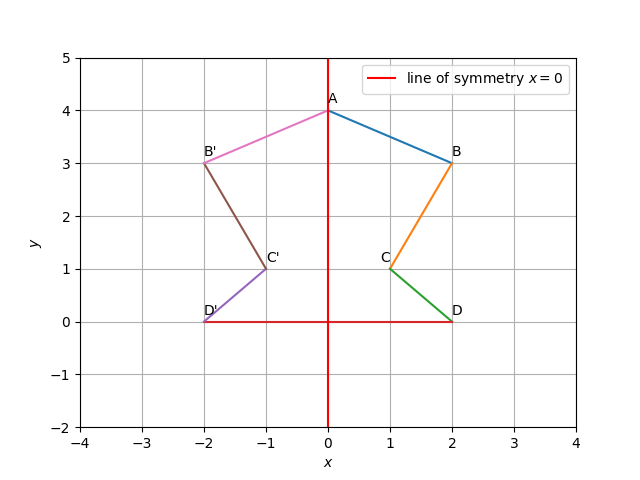
\includegraphics[scale=1.0]{Figure_1.png}
 \end{figure}
 \end{LARGE}
\end{document}